\section{Results}

\subsection{Preselection}

    For the estimators listed in Table~\ref{table:AImethods}, we presented performance score in Table~\ref{table:regression} for regression analysis and in Table~\ref{table:classification} for classification analysis. The results were obtained using the default hyperparameters. \gls{RF}, \gls{ET}, \gls{KN}, \gls{SVM}, and \gls{MLP} estimators predicted the performance metrics with significantly higher accuracy than the others. Even without hyperparameter optimization, \gls{R2} scores of these five estimators ranged from 90 to 98\% for regression and from 92 to 96\% for classification. This implies that the trained models by these estimators will have very low variance. The \gls{ET} regressor most accurately predicted the performance metrics while the \gls{SVM} classifier was superior to the others in classifying designs.

    In general, the linear methods (i.e., \gls{SGD}, \gls{R}, \gls{EN}, \gls{L}, \gls{LL}, \gls{P}, and \gls{Log}) yielded lower fit scores and higher errors with respect to the non-linear methods such as ensemble, \gls{SVM}, and \gls{ANN}. These results clearly imply that linear methods are not quite enough to design a nuclear reactor and thus in predicting its performance metrics. Like linear methods, the \gls{NB} classification methods such as \gls{GNB} and \gls{BNB} seem inappropriate due to the suboptimal performance scores. This is because these methods such as linear and \gls{NB} are not sufficient to fit the training dataset (leading to underfitting) into a linear function due to the higher degree interdependencies of our feature parameters. In addition to this, the \gls{RF}, \gls{DT}, \gls{B}, and \gls{AB} estimators, gave similar results, except for fit score values, as they use the same base estimator (\gls{DT}) in training. Likewise, the \gls{LP} classifier produced the same results with the \gls{SVM} classifier due to the use of the same kernel ($rbf$). In regression analysis, the \gls{ET} regressor has the lowest \gls{MAE} and \gls{MSE} scores while the \gls{R} regressor has the highest scores.

    As to the classification, the \gls{SVM} classifier has the lowest \gls{HL} and \gls{LRL} scores while the \gls{P} classifier has the highest scores. Briefly, any design can be classified with high precision ($>$ 95\%) and very few incorrectly predicted labels (false neagtive plus false positive: $<$ 5\%), leading to an opportunity for an accurate prediction of reactor design even without making any regression analysis.

    On the whole, five estimators (i.e., \gls{RF}, \gls{ET}, \gls{KN}, \gls{SVM}, and \gls{MLP}) that satisfy a score of more than 90\% in \gls{R2} and fit scores appear to be suitable for the subsequent stage of calculations. Among the selected estimators, the \gls{SVM} regressor interestingly shows the second-best performance right after the \gls{ET} regressor despite its worst fit score. In fact, as the scores of the best performing estimators are very close to each other, at this point, it is not easy to distinguish which estimator is the best. Therefore, in the following section, the current scores of these estimators are further improved by tuning their hyperparameters and investigating their learning curves.

%%%%%%%%%%%%%%%%%%%%%%%%%%%%%%%%%%%%%%%%
\begin{landscape}
	\begin{table}[ht!]
		\centering
		\caption{Performance scores of the studied regression methods}
		\begin{tabular}{l>{\columncolor[gray]{0.9}}l>{\columncolor[gray]{0.9}}
				l>{\columncolor[gray]{0.9}}l>{\columncolor[gray]{0.9}}
				l>{\columncolor[gray]{0.9}}lllllllllllllllllllllllllll}
			\hline
			& \textbf{\gls{RF}} & \textbf{\gls{ET}} & \textbf{\gls{KN}} &
			\textbf{\gls{SVM}} & \textbf{\gls{MLP}} & \textbf{\gls{DT}} & \textbf{GB} &
			\textbf{B} & \textbf{AB} & \textbf{SGD} & \textbf{R} & \textbf{EN} &
			\textbf{L} & \textbf{LL} \\
			\hline
			fit score & 1.00 & 1.00 	& 0.99  & 0.96 	& 0.99  & 1.00 & 0.97 & 1.00
			& 0.78	& 0.54 	& 0.73 	& 0.70 	& 0.69 	& 0.55 \\
			EVR  & 0.90 & 0.98 & 0.97 & 0.98 	& 0.95  & 0.90 &
			0.89 & 0.90 & 0.54	& 0.38 & 0.37 & 0.46 & 0.25 & 0.38 \\
			\gls{MAE} & 1.27 & 0.35	& 0.57  & 0.54 	& 0.87  & 1.28 &
			1.72 & 1.27 & 3.36 & 4.77 & 4.78 & 4.60 & 4.77 	& 4.77	\\
			\gls{MSE} & 7.60 & 0.62 & 1.61 & 1.45 & 2.97 & 7.71 & 12.99
			& 7.60 & 38.85 & 82.73	& 82.94	& 77.95	& 81.94	& 82.95	\\
			R$^2$ & 0.90 & 0.98 & 0.97 & 0.98 & 0.95  & 0.90 & 0.89 & 0.90 &
			0.00 & 0.23 & 0.22 & 0.35 & 0.07 & 0.23	\\
			\hline
		\end{tabular}
		\label{table:regression}
	\end{table}
	%%%%%%%%%%%%%%%%%%%%%%%%%%%%%%%%%%%%%%%%
	\begin{table}[ht!]
		\caption{Performance scores of the studied classification methods}
		\begin{tabular}{l>{\columncolor[gray]{0.9}}l>{\columncolor[gray]{0.9}}
				l>{\columncolor[gray]{0.9}}l>{\columncolor[gray]{0.9}}
				l>{\columncolor[gray]{0.9}}llllllllllllllllll}
			\hline
			& \textbf{\gls{RF}} & \textbf{\gls{ET}} & \textbf{\gls{KN}}	&
			\textbf{\gls{SVM}}   & \textbf{\gls{MLP}}& \textbf{\gls{DT}} &
			\textbf{\gls{B}} &
			\textbf{\gls{LP}} & \textbf{\gls{GB}}  & \textbf{\gls{AB}} &
			\textbf{\gls{SGD}}	& \textbf{\gls{R}} &
			\textbf{\gls{GNB}}  & \textbf{\gls{BNB}}& \textbf{\gls{P}}&
			\textbf{\gls{Log}}\\
			\hline
			fit score  	& 1.00 	& 1.00 	& 0.91 	& 0.90 	& 0.90 	& 1.00 	& 0.98 	& 0.90
			& 0.88 & 0.84 	& 0.61 	& 0.65 	& 0.64 	& 0.55 	& 0.45 	& 0.68\\
			\gls{AP} & 0.90 	& 0.93 	& 0.92 	& 0.95 	& 0.96 	& 0.90 	&
			0.90 	& 0.96 	& 0.91 & 0.90 	& 0.80 	& 0.69 	& 0.78 	& 0.52 	& 0.77 	& 0.81\\
			\gls{HL} & 0.05 	& 0.04 	& 0.04 	& 0.03 	& 0.04 	& 0.05 	&
			0.05 	& 0.04 	& 0.05 & 0.06 	& 0.17 	& 0.18 	& 0.13 	& 0.18 	& 0.22 	& 0.17\\
			\gls{LRAPS} & 0.94 	& 0.95 	& 0.95 	& 0.96 	& 0.96 	& 0.94 	& 0.94
			& 0.95 	& 0.94 & 0.93 	& 0.81 	& 0.81 	& 0.86 	& 0.82 	& 0.77 	& 0.82\\
			\gls{LRL} & 0.09 	& 0.07 	& 0.07 	& 0.06 	& 0.06 	& 0.09 	&
			0.09 	& 0.06 	& 0.08 & 0.09 	& 0.27 	& 0.28 	& 0.21 	& 0.27 	& 0.34 	& 0.27\\
			\gls{ROCAUC} & 0.92 	& 0.94 	& 0.94 	& 0.96 	& 0.95 	& 0.92 	&
			0.92 	&
			0.92 	& 0.93 & 0.93 	& 0.79 	& 0.70 	& 0.87 	& 0.60 	& 0.75 	& 0.77\\
			\hline
		\end{tabular}
		\label{table:classification}
	\end{table}
\end{landscape}
%%%%%%%%%%%%%%%%%%%%%%%%%%%%%%%%%%%%%%%%

\subsection{Hyperparameters optimization and learning curve}

    We applied two distinct methods to the estimators to improve their performance. The first method, expected to have an impact on the \gls{R2} scores, prediction errors, and thus cross-validation results, aims to find an optimal size for the training dataset. For this, Figure~\ref{fig:lc} demonstrates the estimator's learning curves for the (U-Th)F$_4$-NaF-BeF$_2$ fuel-salt pair from the viewpoint of \gls{R2} score in regression and multi-label classification accuracy in classification.

    At first look, the \gls{MLP} and \gls{SVM} predictive models do not require more data since the training and cross-validation scores converge together. On the contrary, the \gls{RF}, \gls{ET} and \gls{KN} models require more data as their training scores are much higher than their cross-validation scores.

    From all the learning curves, the \gls{RF}, \gls{ET}, \gls{MLP}, and \gls{SVM} models require a training size in the range of 32000 and 40000 in which the curves level off to a \gls{R2} score of 0.99 whereas the \gls{KN} model requires sample size more than 40000. A similar situation was observed in the classifiers' learning curves. As a result, we decided to use about forty thousand samples for each fuel-salt pair. In other words, for nine fuel-salt pairs, we generated around three hundred thousand samples in total. In the second method, we obtained optimal hyperparameters of the estimators tabulated in Table~\ref{table:hyper}. Parameters not listed in the table are at their default values and do not need optimization.

%%%%%%%%%%%%%%%%%%%%%%%%%%%%%%%%%%%%%%%
    \begin{figure}[ht!]
    	\begin{center}
    		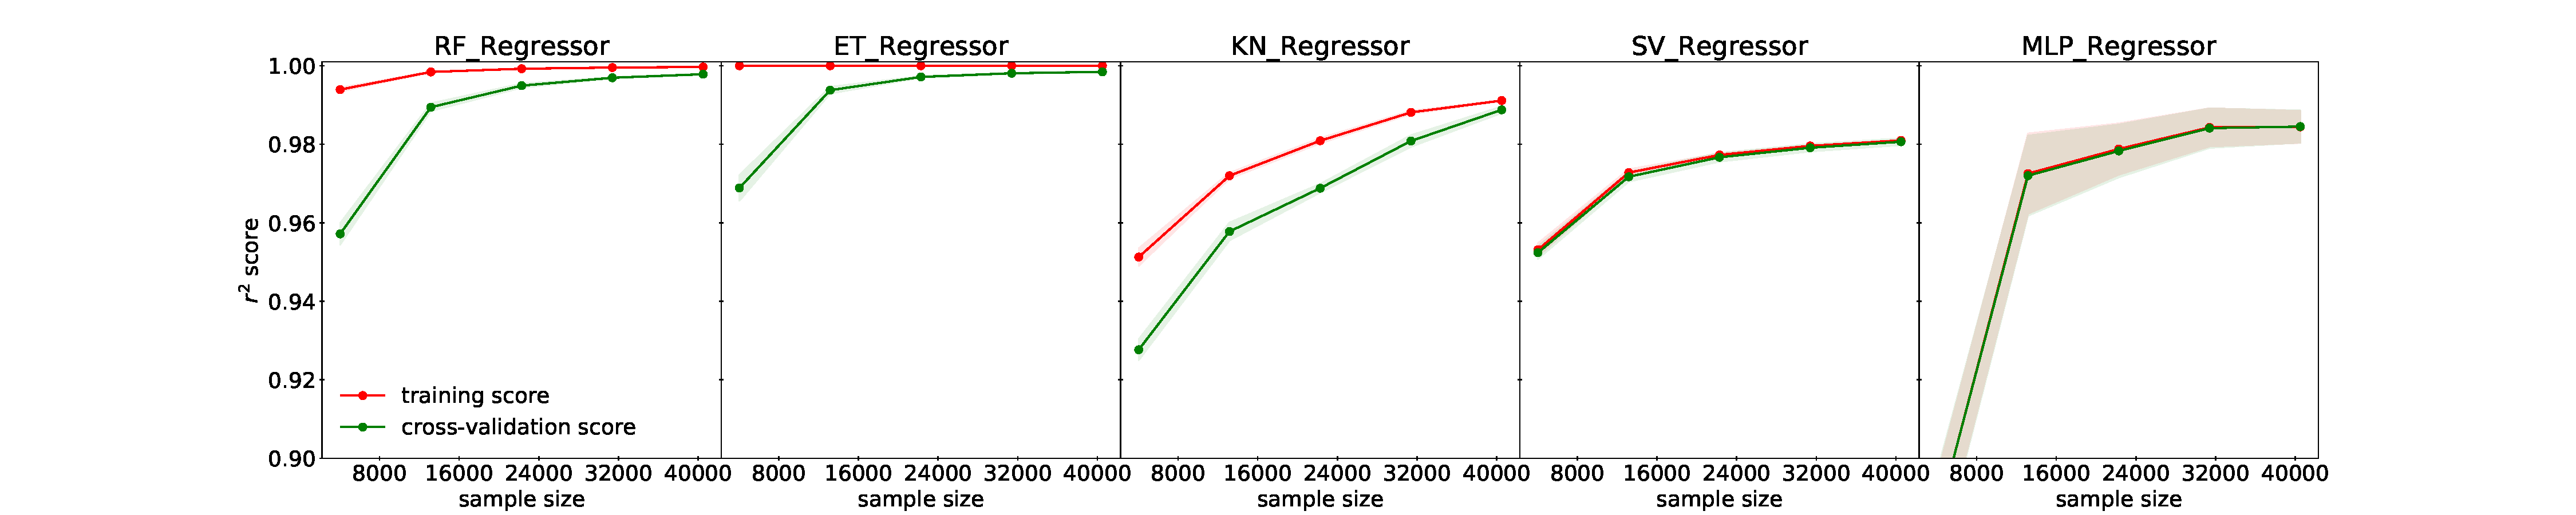
\includegraphics[trim=200 0 200 0, clip,
    		width=\textwidth]{images/regressors_learning_curves.pdf}

    		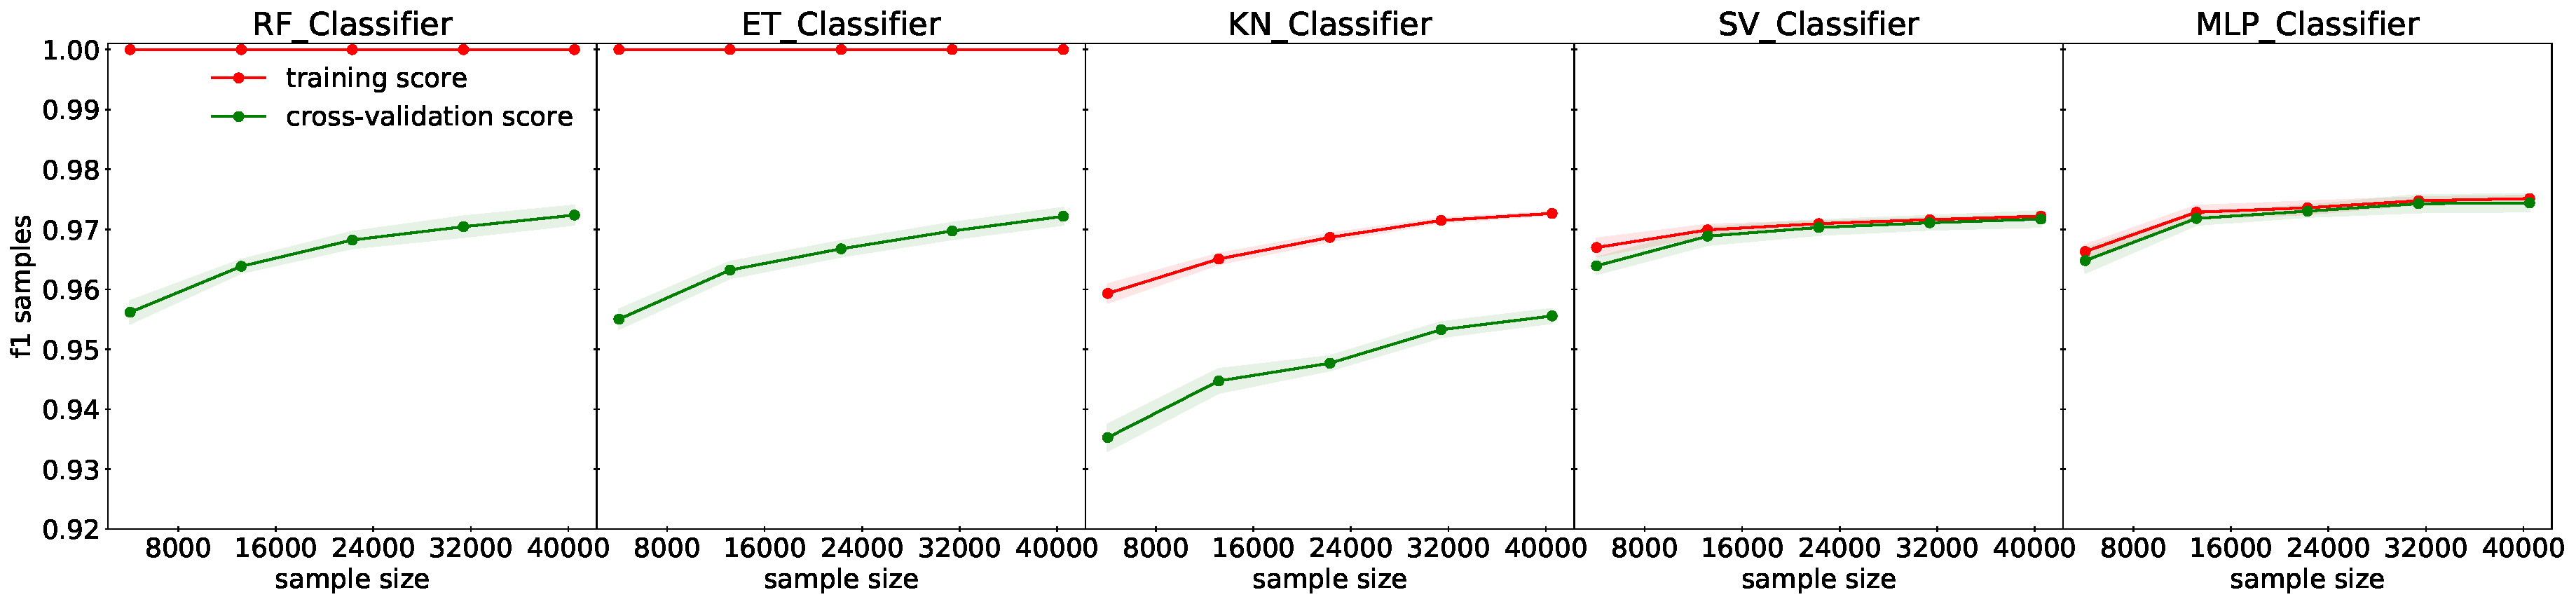
\includegraphics[width=\textwidth]{images/classifiers_learning_curves.pdf}
    	\end{center}
    	\caption{Learning curves of the selected estimators. Solid lines represent mean scores, while the shaded areas around lines represent the standard deviation of the mean due to error.}
    	\label{fig:lc}
    \end{figure}
%%%%%%%%%%%%%%%%%%%%%%%%%%%%%%%%%%%%%%%%
%%%%%%%%%%%%%%%%%%%%%%%%%%%%%%%%%%%%%%%%
\begin{table}[ht!]
	\centering
	\caption{Optimal hyperparameters of the selected estimators}
	\begin{tabular}{l p{0.8\linewidth}}
		\hline
		\textbf{Method} & \textbf{Parameters  (Regressor/Classifier)} \\
        \hline
		\gls{RF} & maximum features: None/None, number of trees: 400/400, minimum number of samples: 7/7                 \\
		\gls{ET} & maximum features: None/None, number of trees: 800/800, minimum number of samples: 1/7, quality criterion: -/gini    \\
		\gls{KN} & weight function: distance/distance, number of neighbors: 7/44, distance metric: manhattan/manhattan, leaf size: 136/200  \\
		\gls{SVM} & kernel type: rbf/poly, polynomial degree: -/3, kernel coefficient: auto/scale, epsilon: 0.1/-, regularization parameter: 3.4/1.2, stopping criterion: 1e-5 \\
		\gls{MLP} & activation function: relu/tanh, hidden layers: 1000/250, maximum iterations: 1e4/1e4, tol: 1e-5, solver: adam/sgd, learning rate: adaptive/constant       \\ \hline
	\end{tabular}
	\label{table:hyper}
\end{table}

\subsection{Final Estimators}

    After performing the hyperparameter optimization and learning curve assessment, we evaluated the final scores of the selected estimators and listed them in Table~\ref{table:finalreg} and ~\ref{table:finalclf}. At a glance, we saw that there is a slight enhancement in the performance scores of all regressors, except for the scores of the \gls{MLP} regressor that exhibits a strong hyperparameter dependency. However, the hyperparameter optimization did not improve the scores of the classifiers. With the optimized hyperparameters and data size in the training dataset, the \gls{ET}, \gls{SVM}, and \gls{MLP} regressors predicted performance metrics with a higher \gls{R2} and lower \gls{MAE} compared to their preselection scores.

    On the other hand, the \gls{SVM} and \gls{MLP} classifiers labeled the design attributes with the highest \gls{AP} and lowest \gls{LRL} scores relative to the other estimators. Nonetheless, the others are also suitable as all the scores are very close to each other. As the scores did not give us sufficient information about determining the right estimator for the next phase, we investigated cross-validation plots and multi-label confusion matrices on the basis of each performance metric (i.e., $k_{\infty}$, $\varsigma$, $\phi_{fast}$).

%%%%%%%%%%%%%%%%%%%%%%%%%%%%%%%%%%%%%%%%
    \begin{table}[ht!]
    	\centering
    	\caption{Final performance scores of the selected regressors}
    	\begin{tabular}{lllll>{\columncolor[gray]{0.9}}l}
    		\hline
    		& \textbf{\gls{RF}}  & \textbf{\gls{ET}}  & \textbf{\gls{KN}} &
    		\textbf{\gls{SVM}}   & \textbf{\gls{MLP}} \\
    		\hline
    		fit score  & 1.00 	& 1.00 & 1.00 & 0.97  & 1.00 \\
    		\gls{EVR} & 0.94 & 0.99 & 0.99 & 0.96 & 1.00 \\
    		\gls{MAE} & 1.07 & 0.28 & 0.41 & 0.37 & 0.23 \\
    		\gls{MSE} & 5.52 & 0.41 & 0.83 & 0.44 & 0.24 \\
    		R$^2$ & 0.94 & 0.99 & 0.98 & 0.96 & 1.00 \\
    		\hline
    	\end{tabular}
    	\label{table:finalreg}
    \end{table}
%%%%%%%%%%%%%%%%%%%%%%%%%%%%%%%%%%%%%%%%
    \begin{table}[ht!]
    	\centering
    	\caption{Final performance scores of the selected classifiers}
    	\begin{tabular}{lllll>{\columncolor[gray]{0.9}}l}
    		\hline
    		& \textbf{\gls{RF}} & \textbf{\gls{ET}}  & \textbf{\gls{KN}} &
    		\textbf{\gls{SVM}}  & \textbf{\gls{MLP}} \\
    		\hline
    		fit score  & 0.93 & 1.00 & 1.00  & 0.89 & 0.90 \\
    		\gls{AP} & 0.92 & 0.94 & 0.95  & 0.96 & 0.97  \\
    		\gls{HL} & 0.04 & 0.04 & 0.04  & 0.03 & 0.03  \\
    		\gls{LRAPS}  & 0.95 & 0.96 & 0.96  & 0.96 & 0.97 \\
    		\gls{LRL} & 0.07 & 0.06 & 0.06  & 0.05 & 0.05  \\
    		\gls{ROCAUC} & 0.94 & 0.95 & 0.96  & 0.95 & 0.96 \\
    		\hline
    	\end{tabular}
    	\label{table:finalclf}
    \end{table}
%%%%%%%%%%%%%%%%%%%%%%%%%%%%%%%%%%%%%%%%

\subsection{Cross-validation plot and confusion matrix}

    In this section, we compared the predicted test dataset with the actual test dataset. Figure~\ref{fig:cv} visualizes the predicted performance metrics against their actual values for the chosen estimators in terms of cross-validation plots. These plots show the estimator's prediction quality separately for each performance metric. Results indicated that the \gls{ET}, \gls{KN}, and \gls{MLP} estimators accurately predict performance metrics per the acceptance criterion (within $<$5\% relative error).

    According to these results, the \gls{ET} estimator is the best option to employ in the optimization phase. In comparison to the actual values, it correctly estimated the $k_{\infty}$ metric, slightly underestimated the $\varsigma$ metric, and predicted a few values of the $\phi_{fast}$ metric outside of the region. The \gls{KN} and \gls{MLP} estimators have good results comparable to the \gls{ET} and, therefore, be considered as alternative estimators for regression analysis.

    For classification analysis, we presented confusion matrices, normalized over the total test sample size, in Figure~\ref{fig:cm} to compare the predicted labels with the actual labels in terms of true/false positive and true/false negative scores. From the prediction capability standpoint, these estimators have very close scores in each label and predict all labels with high precision ($<$95\%). Related to the scores of the labels, the only label that causes the highest misclassification score by 10\% is the feedback coefficient. This mislabeling originates from the feedback coefficients very close to zero as they are not accurately estimated. Other labels were, however, correctly estimated with an error of less than 1\%. As a result, any of these classifiers can easily handle the classification of channel designs without causing a notable loss in labeling. In this context, as in the regression analysis, we decided to use the \gls{ET} classifier in the design optimization phase to estimate the labels of optimum designs.

    \begin{figure}[ht!]
     \begin{center}
            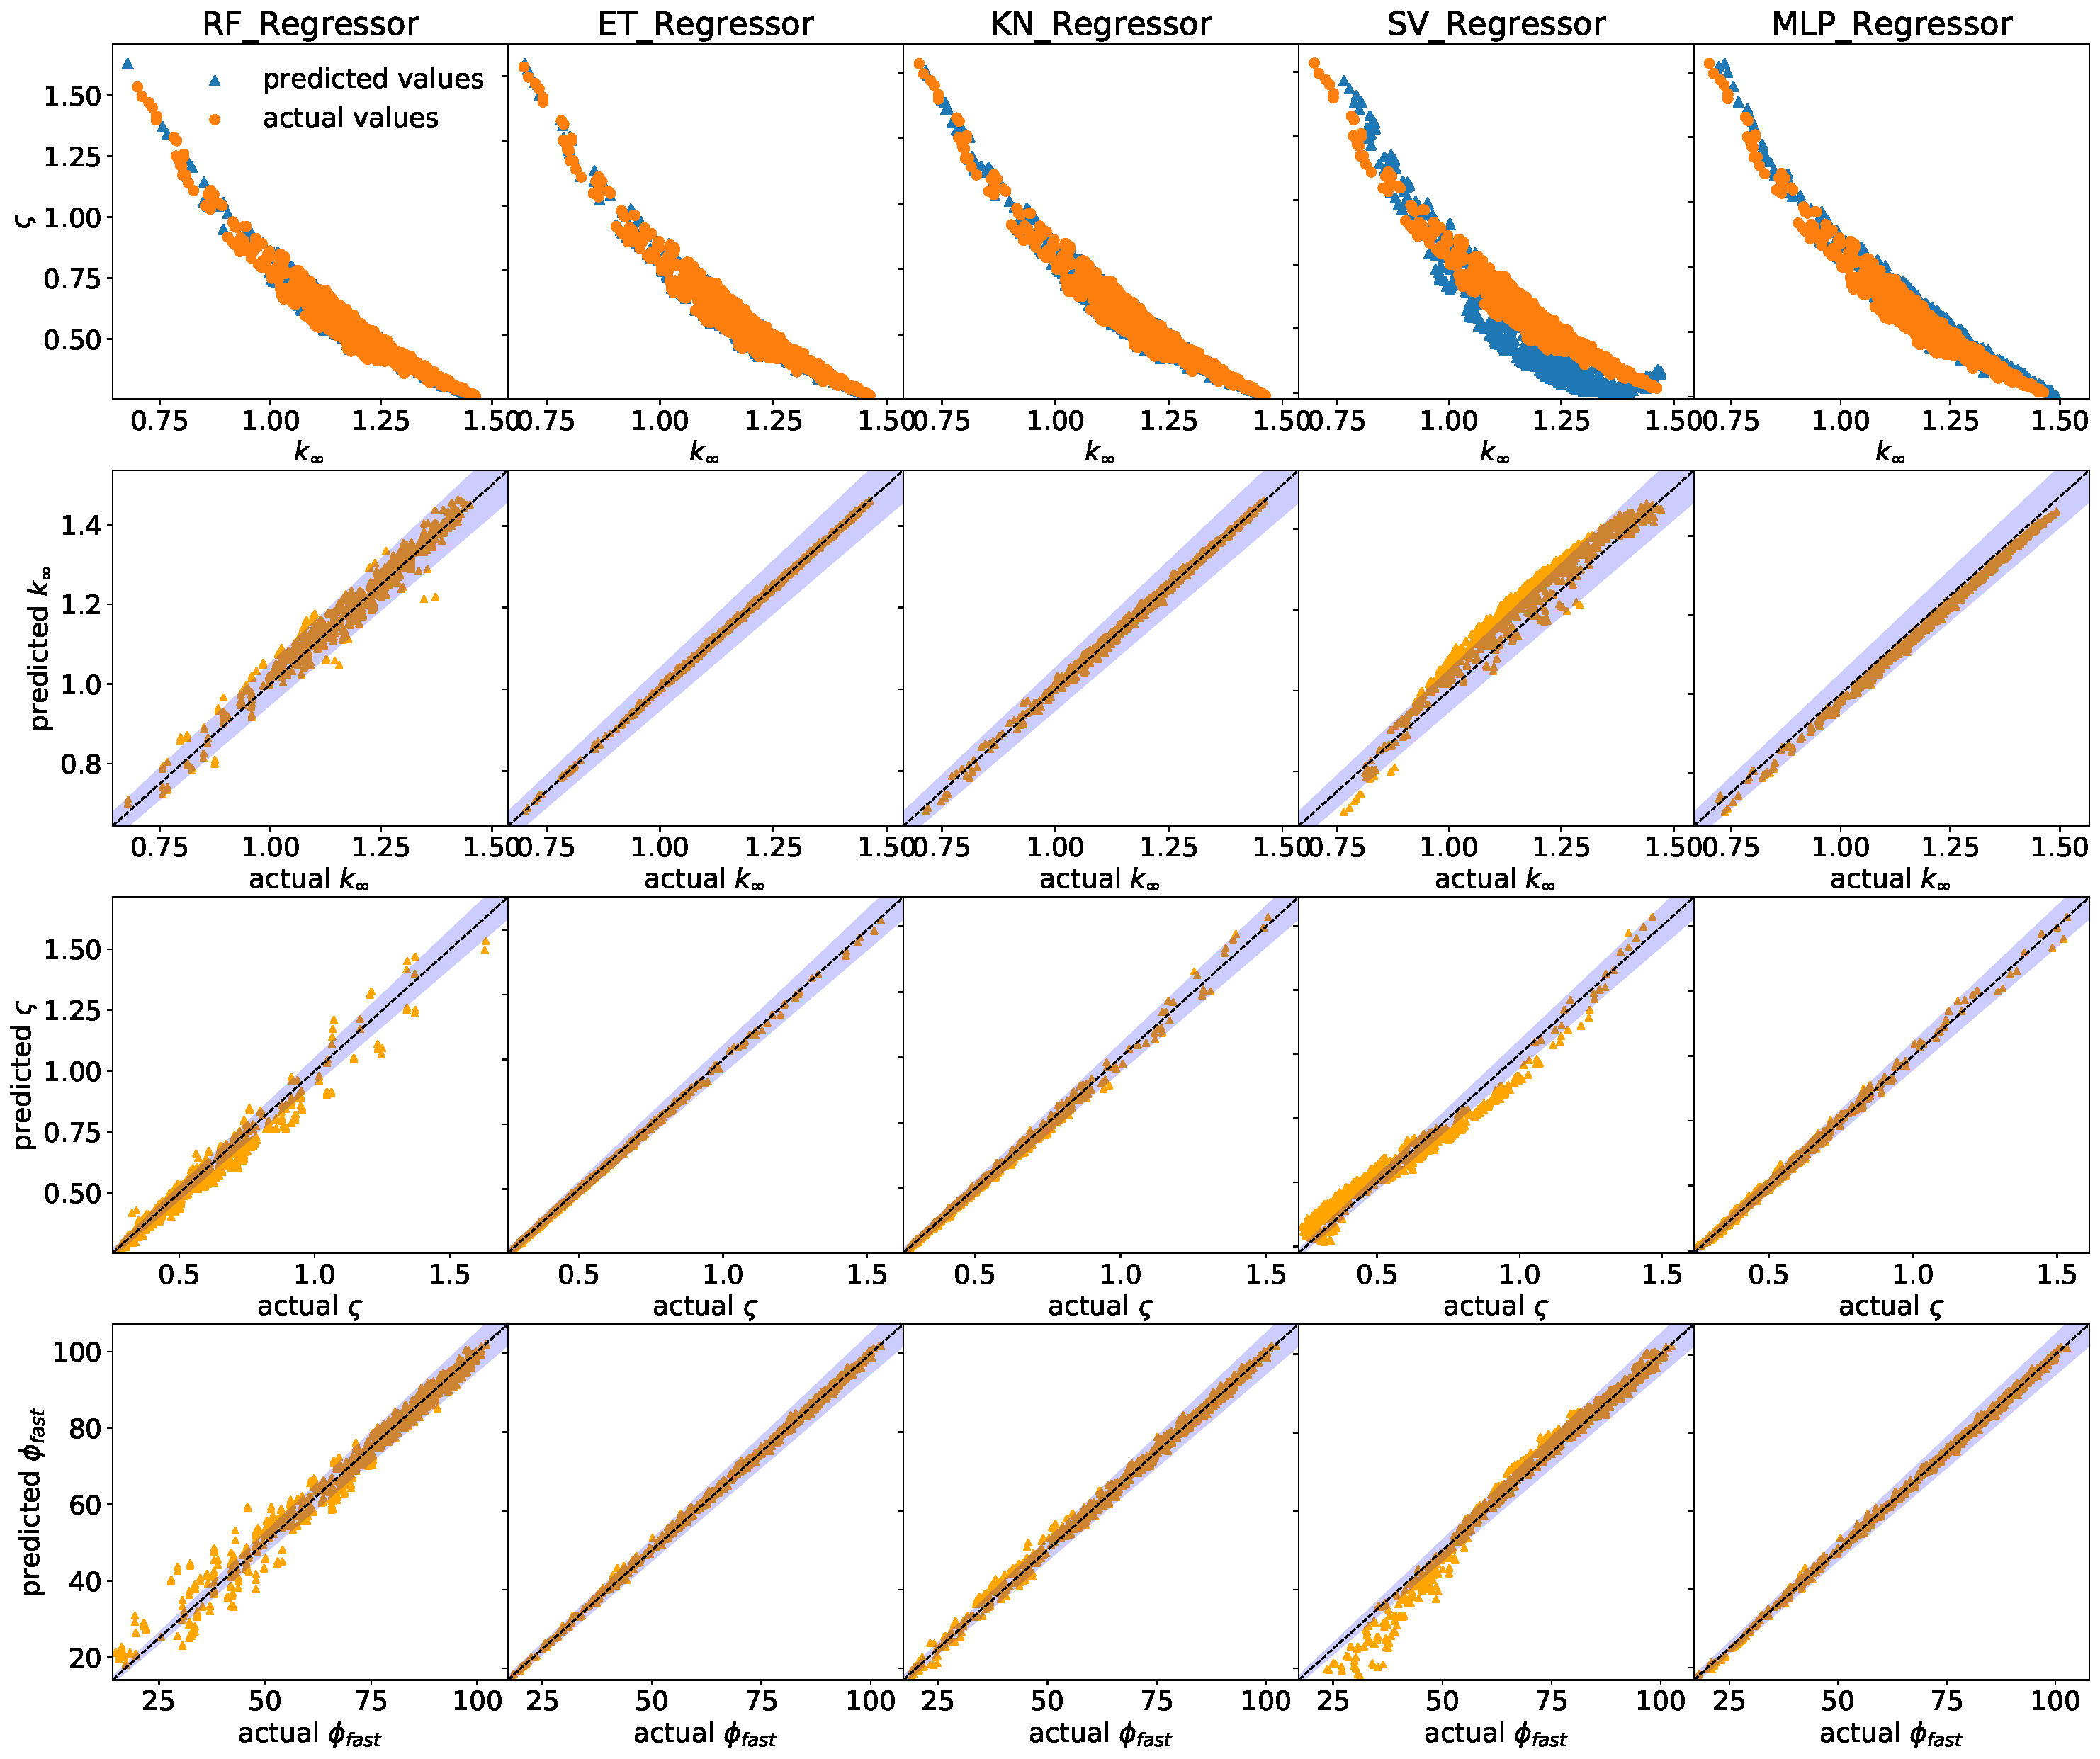
\includegraphics[width=\textwidth]{images/regression_cross_validation.pdf}
     \end{center}
        \caption{Cross-validation plots of the selected regressors, top to bottom:	(i)$k_{\infty}$ versus $\varsigma$ (ii) $k_{\infty}$ (iii) $\varsigma$ and	(iv) $\phi_{fast}$  }
        \label{fig:cv}
    \end{figure}
    \begin{figure}[htbp!]
     \begin{center}
            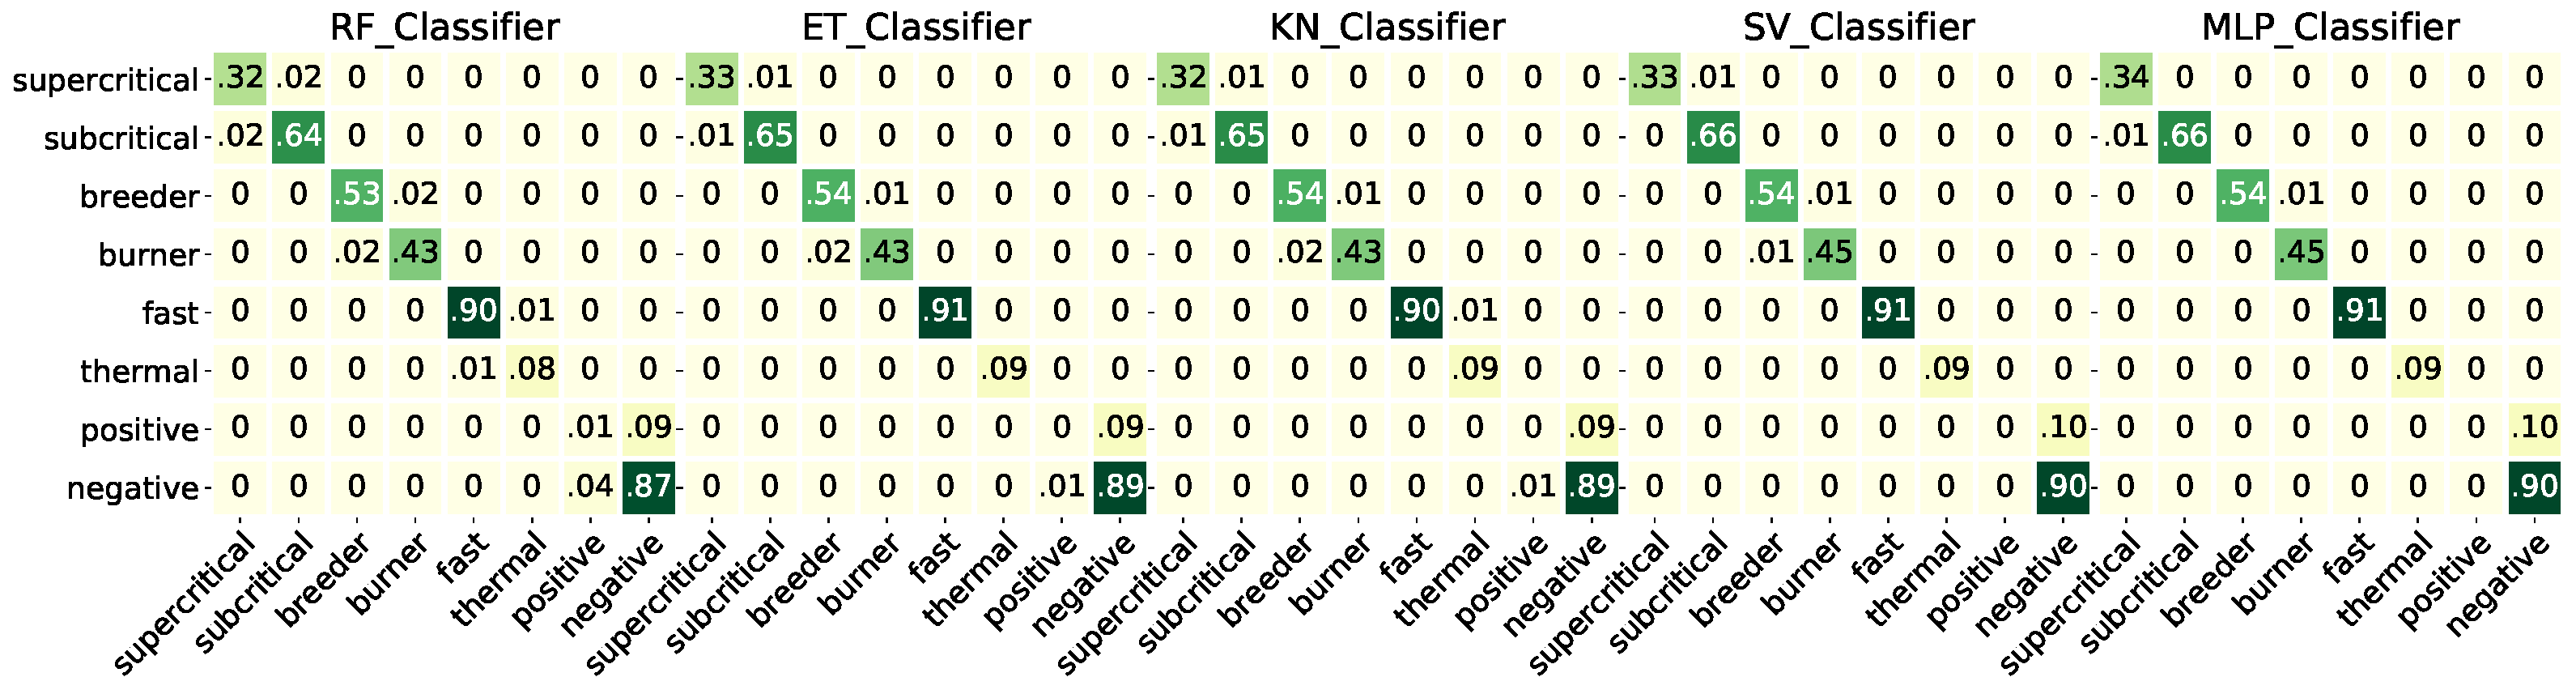
\includegraphics[width=\textwidth]{images/classification_confusion_matrix.pdf}
     \end{center}
        \caption{Normalized confusion matrices of the selected classifiers}
        \label{fig:cm}
    \end{figure}

\subsection{Optimum Designs}

    Based on the constraints applied to performance metrics, we found a set of optimum solutions for each fuel-salt pair. As an illustration, we presented the Pareto-front solutions for the (U-Th)F$_4$-NaF-BeF$_2$, which is very similar to the results of other fuel-salt pairs, in Figure~\ref{fig:pareto}. This figure includes (a) cross-validation plots for each performance metric, (b) the distribution of the Pareto-front solutions in 3-D performance metric space, and (c) the normalized confusion matrix. As seen from the subplot (a), the Pareto-optimal solutions (blue triangle) overlapped very well with the actual values (orange circles). The other subplots also confirm this situation by showing good distributions in the very proximity of the intersection line of each performance metric.

    The cross-validation subplots also indicated that all the predicted metrics totally stay within the 5\% relative error (shaded area) and very close to the intersection line. We found even better results for the $k_{\infty}$ metric with no more than 1\% relative error.

    As in the regression analysis results, the classification results of the optimal solutions in subplot (c) agreed very well with the actual labels. The only noteworthy complication is the misclassification of a tiny fraction of the feedback indicators. This mislabeling certainly arose from the prediction of the ${\alpha_{total}}$ values as discussed before and were estimated as positive instead of negative. In conformity with the constraints applied to performance metrics in the optimization phase, all the optimum designs we found are of characteristics of supercritical eigenvalue, fast spectrum, burner type, and negative feedback.

    Of the entire Pareto front solutions (around 650) which account for each combination of the fuel-salt pairs, only the nine best solutions are tabulated in Table~\ref{table:optimaldesigns}. We simply opted for the solutions that grant the highest breeding ratio ($\varsigma$) and the lowest fast flux ($\phi_{fast}$) at the $k_{\infty}$ = 1.06. The only exception for the multiplication factor criterion is for the NaCl salt in U-Pu fuel as there are no solutions with a multiplication factor less than 1.21 for this fuel-salt pair.

    As provided in the table, the suggested solutions can be grouped more easily by fuel type as the solutions show a certain relationship with the fuel type rather than the salt type. When the fuel types are compared to each other, U-Th fuels require the highest $^{235}$U content (18-20\%) due to the existence of the $^{232}$Th isotope which has an absorption cross-section approximately four times higher than $^{238}$U. U fuels reach their top performance when a moderate amount of $^{235}$U (14-15\%) is used. U-Pu fuels need the lowest amount of $^{235}$U (5\%) as not only does Pu in U-Pu already contain a certain fraction of fissile isotopes like $^{239}$Pu and $^{241}$Pu, but also Pu fissile isotopes emit greater average fission neutrons per absorption. Similarly, we noticed that U-Th fuels demand 13-14\% Th in U-Th while U-Pu fuels favor the highest grade of U content (90\%).

    A comprehensive look at the common properties of the optimal designs suggests that $T_{ave}$ should be in the range of 1100-1200 K and $\xi$ needs to be at its minimum value (0.274). Furthermore, as expected, Th necessitates higher fissile material than any other fuel types whereas the fissile material required by the U-Pu fuel is the lowest as the weapons-grade Pu comprises a gread deal of fissile isotopes by almost 50\% of its content. On the other hand, unlike the other feature parameters that display a direct characteristic relationship with the fuel type, there is no noticeable evidence to associate the channel-to-channel pitch length ($p$) with the fuel types. The $p$ parameter is, however, likely to vary with the salt type just as the NaCl salt calls for a constant pitch value of 1.0 cm in all fuel types.

    In summary, among the optimal designs, it appears that all the fuels mixed with the NaCl salt are the most promising designs. In particular, the F$_4$-PuF$_3$-NaCl fuel-salt yields the highest $\varsigma$ and $k_{\infty}$. The most unfavorable side of this fuel-salt is to have a lower ${\alpha_{total}}$ than other salt types but the coefficient is still quite sufficient compared to the exiting designs of \gls{MSR}s at the initial state with a total fuel-salt feedback coefficient of around -3.4 pcm/K \cite{rykhlevskii2019, robertson1971}. From the reactor safety point of view, the LiF-BeF$_2$ salt with the highest ${\alpha_{total}}$ is the most favorable.

    \begin{figure*}
    	\begin{center}
    		\begin{minipage}{.49\linewidth}
    			\begin{subfigure}[t]{1.0\linewidth}
    				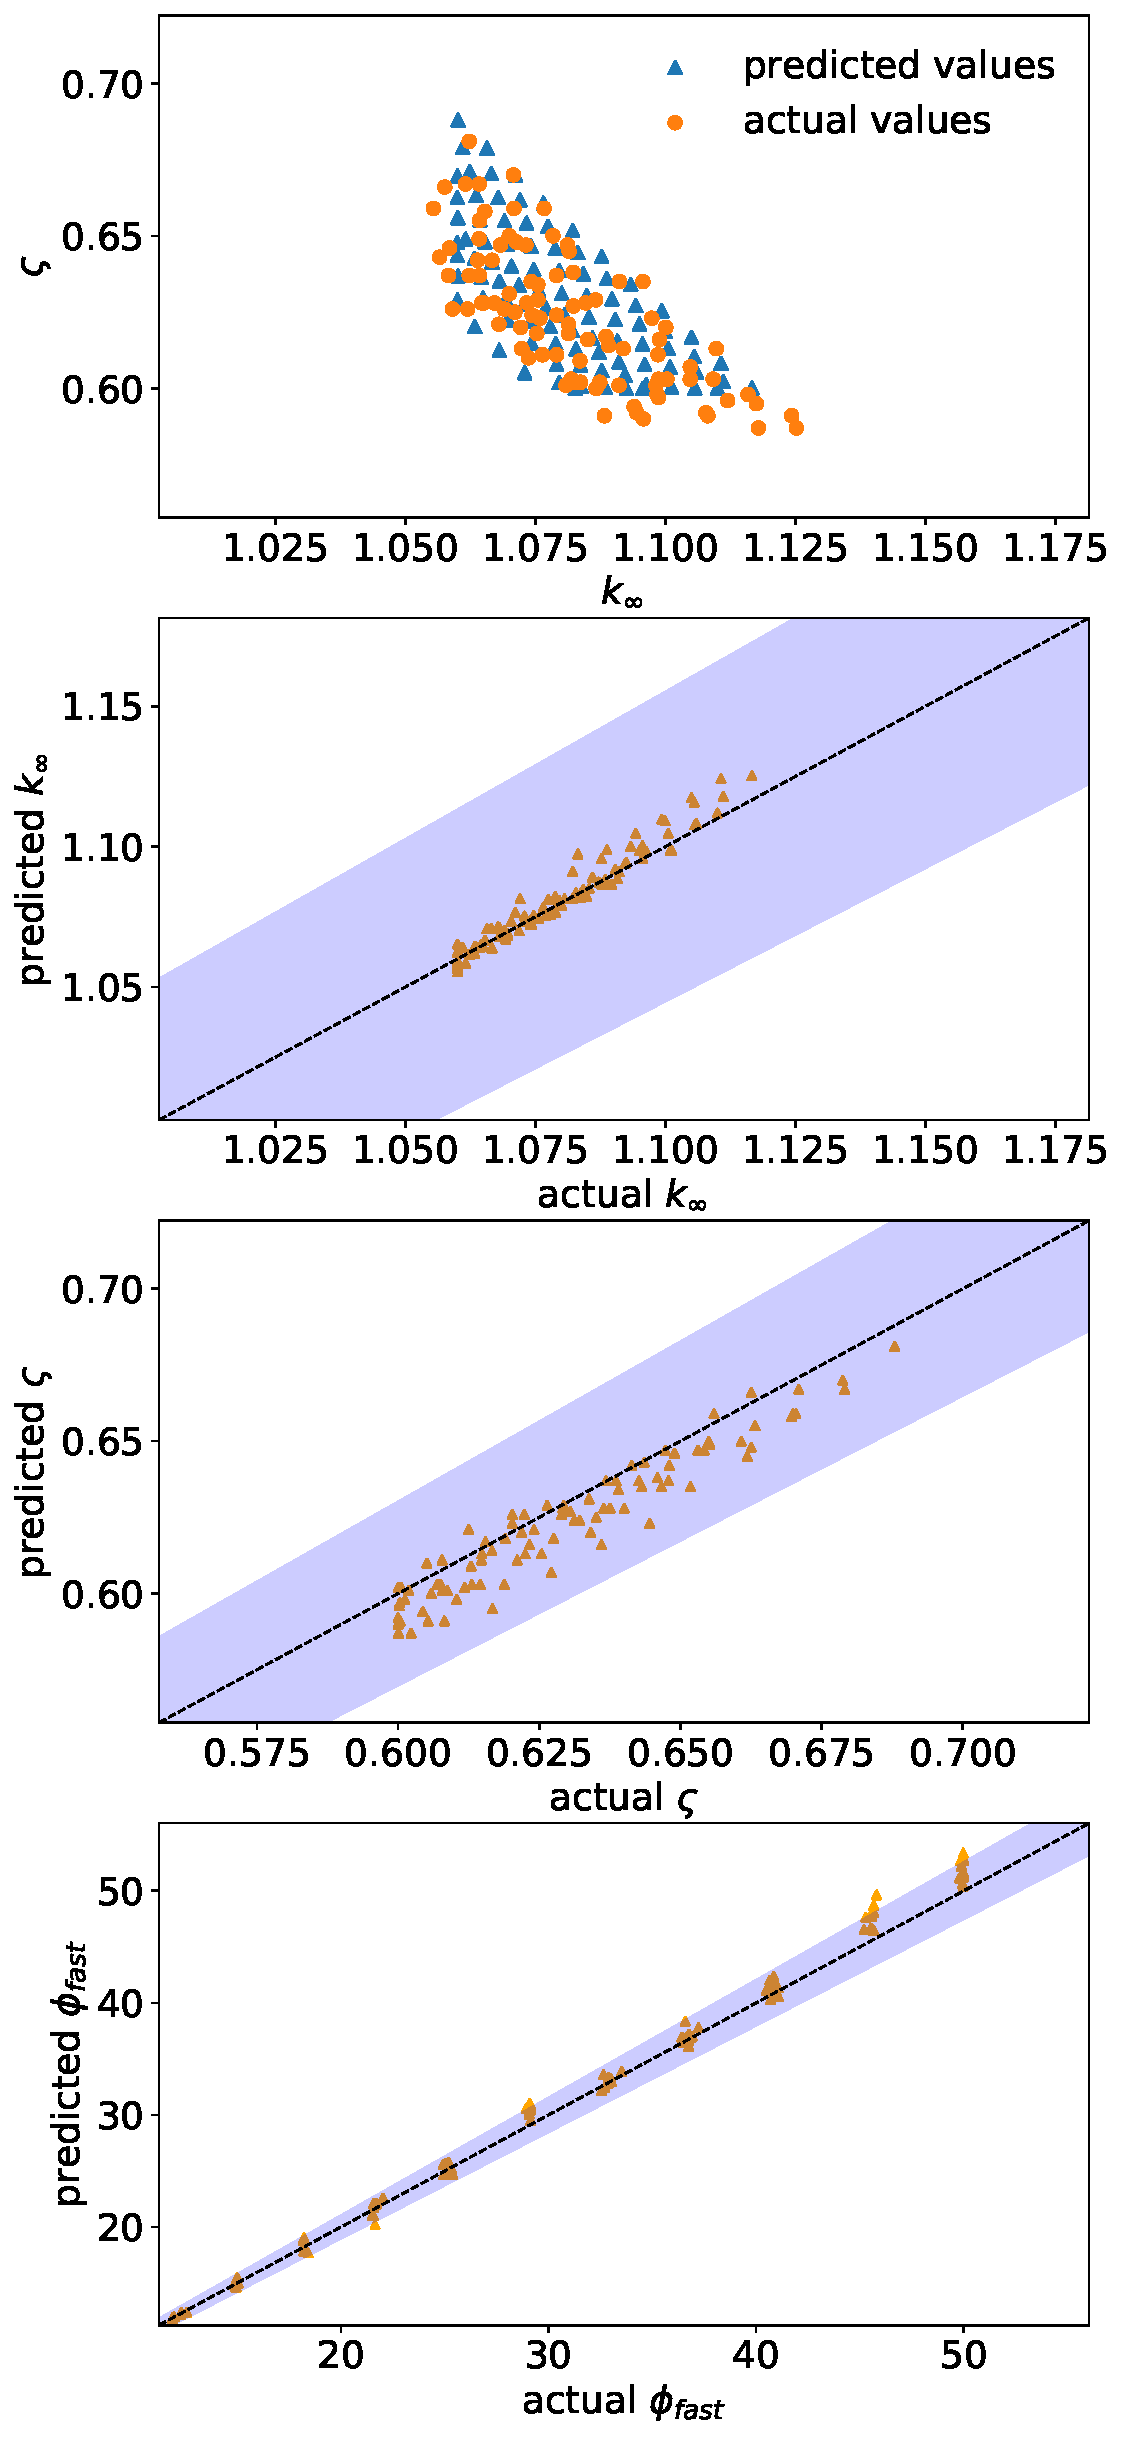
\includegraphics[width=\textwidth]{images/22_optimal_design_cross_validation.pdf}
    				\caption{}
    			\end{subfigure}
    		\end{minipage}
    		\begin{minipage}{.49\linewidth}
    			\begin{subfigure}[t]{1.0\linewidth}
    				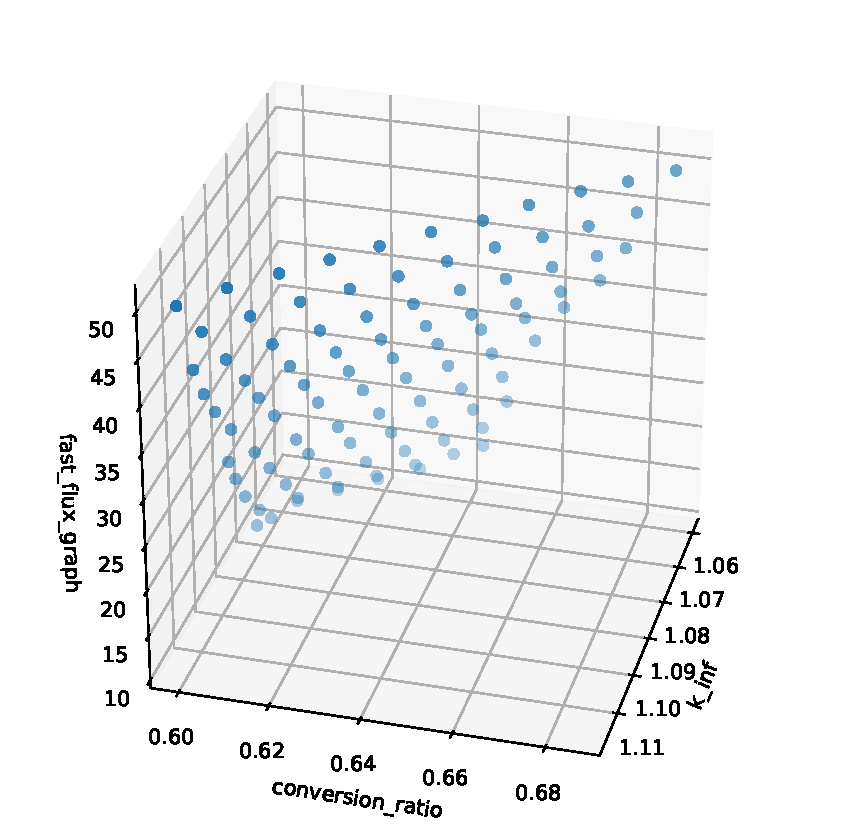
\includegraphics[width=\textwidth]{images/22_optimal_design_3d_solutions.pdf}
    				\caption{}
    			\end{subfigure} \\
    			\begin{subfigure}[b]{1.0\linewidth}
    				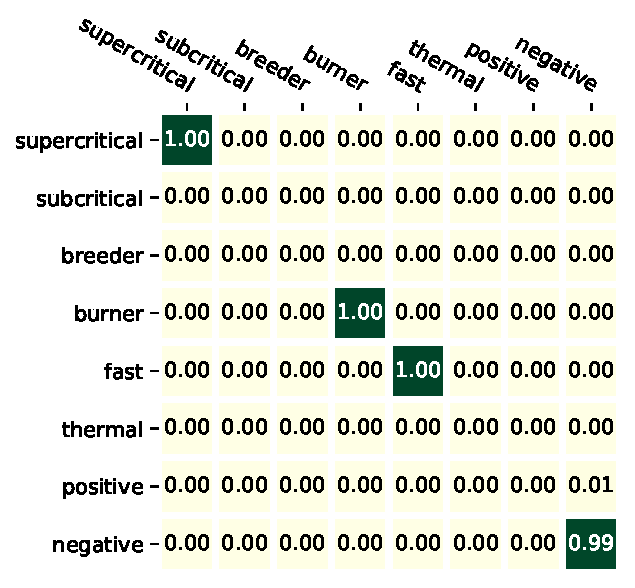
\includegraphics[width=\textwidth]{images/22_optimal_design_confusion_matrix.pdf}
    				\caption{}
    			\end{subfigure}
    		\end{minipage}
    	\end{center}
    	\caption{Optimum solutions for (U-Th)F$_4$-NaF-BeF$_2$: (a) cross-validation plots of performance metrics, (b) the distribution of the Pareto-front solutions in 3-D performance metric space, and (c) the normalized confusion matrix.}
    	\label{fig:pareto}
    \end{figure*}


%%%%%%%%%%%%%%%%%%%%%%%%%%%%%%%%%%%%%%%%
\begin{landscape}
	\begin{table}[ht!]
		\centering
		\caption{Optimal designs for each fuel-salt pair$^\star$}
		\begin{threeparttable}[t]
			\begin{tabular}{lllllllllll}
				\hline
				\textbf{Fuel Type} & \textbf{Salt Type}  & \textbf{$f_{35}$} &
				\textbf{$f_{U}$} & \textbf{$p$}	& \textbf{$T_{ave}$} & \textbf{$\xi$} &
				\textbf{$k_{\infty}$ \tnote{$\dagger$}}	& \textbf{$\varsigma$
					\tnote{$\ddagger$}}  & \textbf{$\phi_{fast}$ \tnote{$\perp$}} &
				\textbf{${\alpha_{total}}$ 	\tnote{$\wedge$}}  \\
				\hline

				U 	& LiF-BeF$_2$ 	& 14.47 & 100.0 & 86.7 & 1200 & 0.274 & 1.0600(+60) &
				0.661(-6) & 18.6(-0.5) 	& -3.9\\
				U 	& NaF-BeF$_2$ 	& 14.88 & 100.0 & 7.18 & 1125 & 0.274 & 1.0600(-120) &
				0.638(+6) & 19.0(-0.9) 	& -4.0\\
				U 	& NaCl 	& 14.28 & 100.0 & 1.00 & 1176 & 0.274 & 1.0604(-20) &
				0.692(0) & 12.6(0) 	& -3.0\\
				U-Th & LiF-BeF$_2$ 	& 19.10	& 86.7 & 5.50 & 1123 & 0.276 & 1.0601(-70) &
				0.665(-7) & 17.1(-0.2) 	& -4.3\\
				U-Th & NaF-BeF$_2$ 	& 20.00 & 86.8 & 5.98 & 1125 & 0.275 & 1.0600(+30) &
				0.643(-11) & 16.0(-0.2) & -2.8\\
				U-Th 	& NaCl 	& 18.48	& 86.2 	& 1.00 	& 1199 & 0.274 & 1.0600(+140) 	&
				0.696(-1) & 14.4(0)	& -2.8\\
				U-Pu & LiF-BeF$_2$ 	& 5.00 	& 90.0 	& 4.40 	& 1198 & 0.274 & 1.0600(-20) &
				0.732(+3) & 16.0(0.2) & -4.5\\
				U-Pu	& NaF-BeF$_2$ 	& 5.00 	& 89.3 & 4.37 & 1125 & 0.275 & 1.0600(+460) &
				0.723(+15) & 13.6(0.3) 	& -3.3\\
				U-Pu	& NaCl & 5.00 & 90.0 & 1.00 & 1193 	& 0.274 & 1.2192(+10) &
				0.753(+1) & 13.0(0)	& -3.4\\
				\hline
			\end{tabular}
            \rule{0in}{1.2em}$^\star$\scriptsize Performance metrics given in the table are the predicted values. The values inside the brackets are the actual values in terms of difference from the predicted values.

			\rule{0in}{1.2em}$^\dagger$\scriptsize The computational error of the infinite multiplication factor is $\pm$0.0009. The values within the brackets are in the units of pcm.

			\rule{0in}{1.2em}$^\ddagger$\scriptsize The computational error of the conversion ratio is $\pm$0.005. The values within the brackets are in the units of milli.

			\rule{0in}{1.2em}$^\perp$\scriptsize The computational error of the fast flux is $\pm$0.007.

			\rule{0in}{1.2em}$^\wedge$\scriptsize The propagated computational error of the feedback coefficient of reactivity is $\pm$0.4.

		\end{threeparttable}
		\label{table:optimaldesigns}
	\end{table}

\end{landscape}

%%%%%%%%%%%%%%%%%%%%%%%%%%%%%%%%%%%%%%%%
